\subsection{Memcached-silo}
\label{sec:mcdsilo}

Memcached-silo is a workload built on top of the normal memcached protocol. It is computationally and memory more intensive than regular memcached as it incorporates both latency-sensitive network compute and memory-intensive TPC-C style transaction processing. The workload is structured such that every single memcached request triggers a corresponding set of fixed TPC-C transaction processing logic on a in-memory database~\cite{silo}. We ported the memcached-silo implementation~\cite{mcdsilo, zygos} to our libOS. The workload mix and SLA constraints of memcached-silo follow from those used in the memcached experiments. Given its computationally heavier nature, we only needed two 16-core client nodes at 16 connections per core to saturate a single 16-core memcached-silo server. 

\begin{figure*}
\centering
%\vspace*{-0.3cm}  
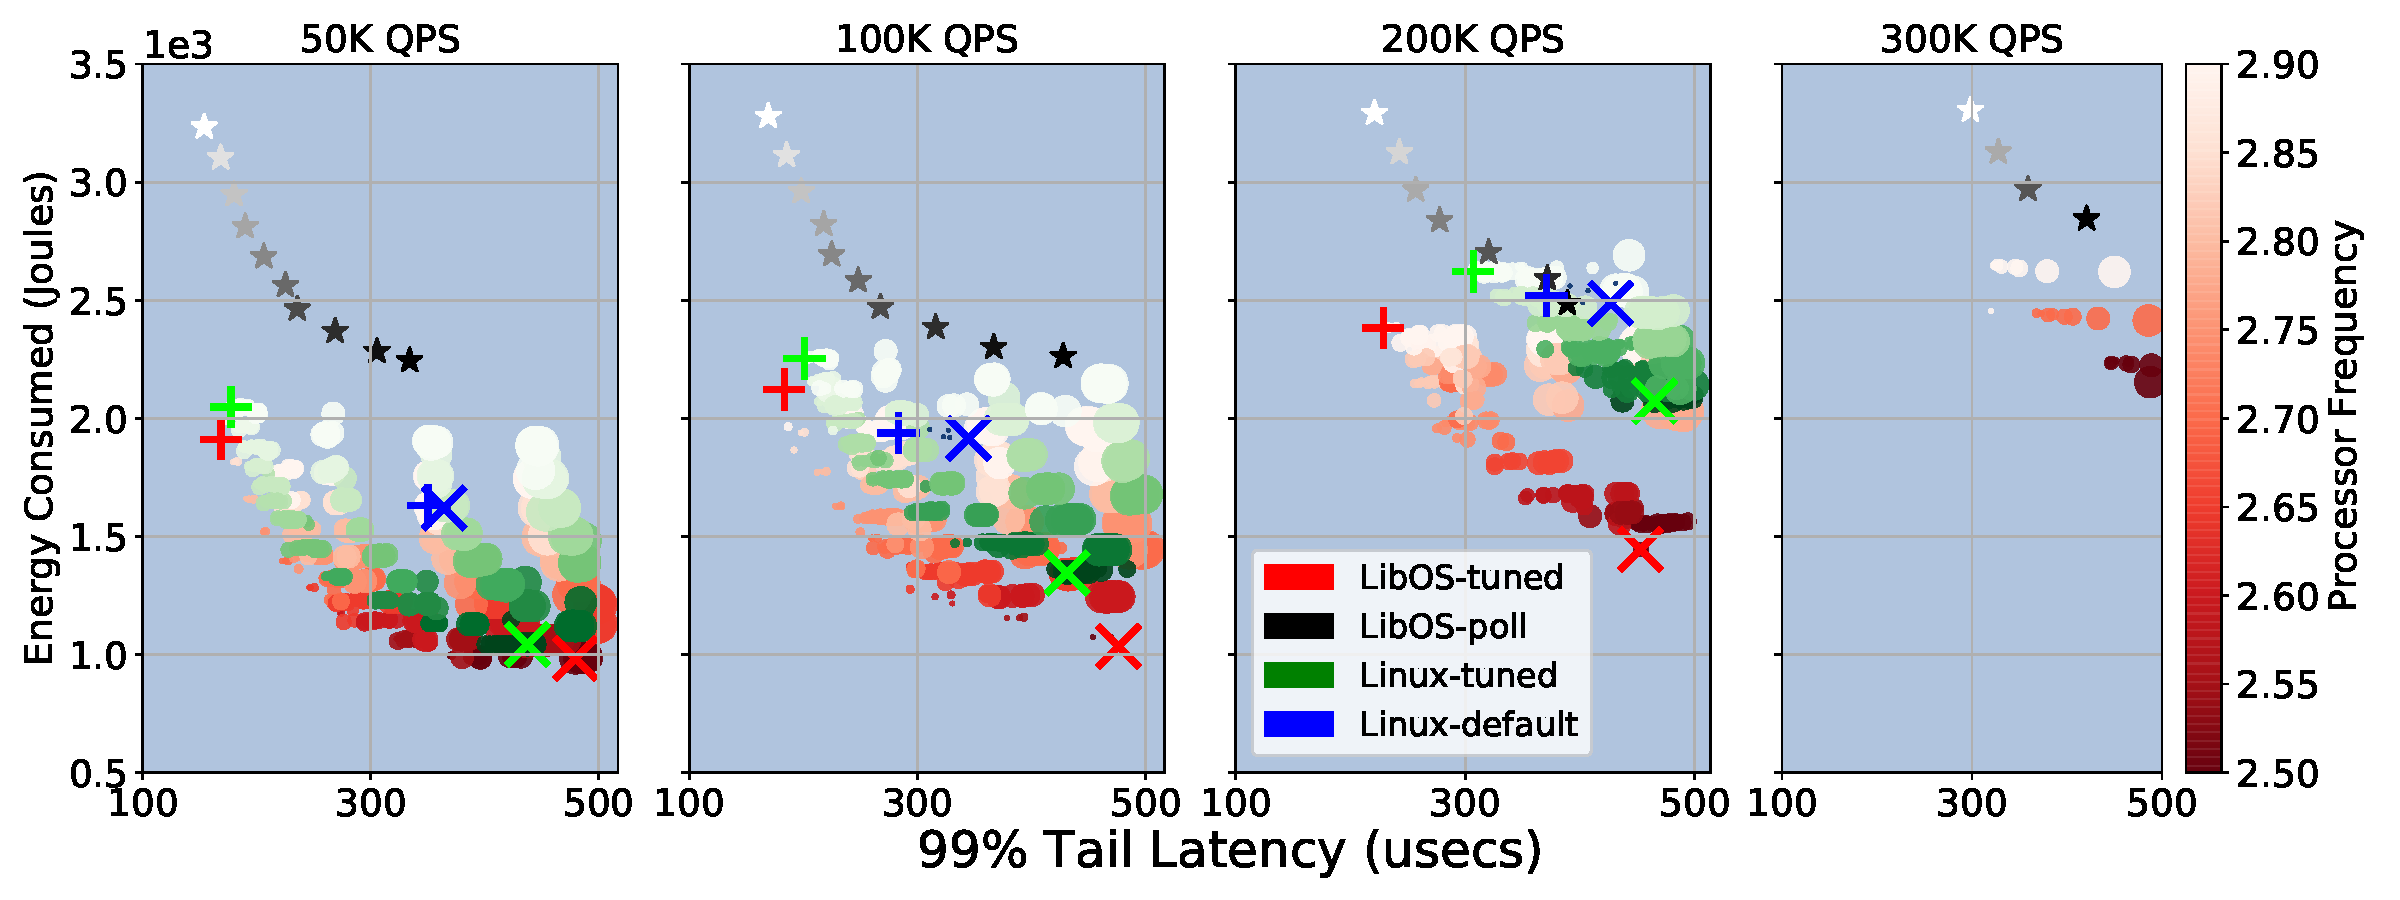
\includegraphics[width=1\textwidth]{figures/mcdsilo_overview}
\caption[]
%{\small 
{Memcached-silo across different QPS.}
\label{fig:mcdsilo_overview}
\end{figure*}

\subsubsection{Finding-1: Implications of OS path length efficiency}
